\documentclass[17pt]{beamer}
% \usepackage{color}
\usepackage{graphicx}
% \usepackage[all,cmtip]{xy}
\usepackage{tikz}
\usepackage{tikz-cd}
\usepackage{amsfonts}
\usepackage{amssymb}
\usepackage{amsmath}
\usepackage{amscd}
\usepackage{amsthm}
\usepackage{bbm}
%\usepackage{pictexwd,dcpic}
% \usepackage[mathcal]{euscript}
\usepackage[utf8]{inputenc}
%\usepackage[T1]{fontenc}
% \usepackage{lmodern}
\title{The Invariant Structure of Equivalent Theories}
\author{Hans Halvorson}
\date{April 23, 2015}
% \usetheme{Default}
% \usetheme{Singapore}
\setbeamertemplate{navigation symbols}{}%remove navigation symbols
% \usetheme{Singapore}
\usepackage{eucal}
\setbeamercolor{normal text}{fg=black,bg=white}
\setbeamercolor{alerted text}{fg=red}
\setbeamercolor{example text}{fg=black}
\usepackage[absolute,overlay]{textpos}
\begin{document}

\def\2{\mathcal}
\def\7{\mathfrak}
\begin{frame}

\maketitle

\end{frame}

\begin{frame}{The hunt for artifact-free representations}

\begin{enumerate}
\item Example: coordinate free geometric theories 
\item Example: comparativism about quantity 
\end{enumerate}

\end{frame}

\begin{frame}{The model isomorphism criterion for theoretical
    equivalence (IC)}

\begin{exampleblock}{}
  $T$ and $T'$ are equivalent only if their models are isomorphic.
\end{exampleblock}

\end{frame}

\begin{frame}

  ``Hamiltonian and Lagrangian mechanics are not equivalent in terms
  of statespace structure.  This means that they are not equivalent,
  period.'' (J.\ North)


\end{frame}

\begin{frame}{The trouble with IC}

  The notion of isomorphism is relative to a species of mathematical
  structure.


\end{frame}

\begin{frame}{Example}

\begin{itemize}
\item Linear orderings in signature $\{ < \}$.
\item Linear orderings in signature $\{ \leq \}$. 
\end{itemize}


\end{frame}

\begin{frame}{Example}


\begin{center}
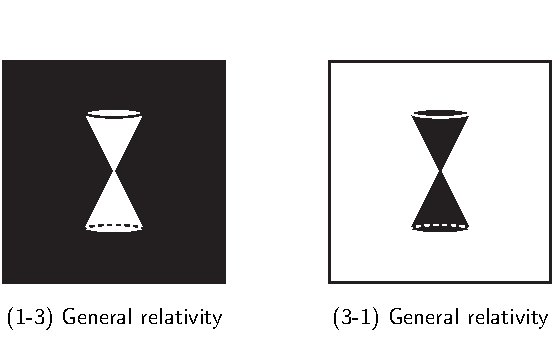
\includegraphics{1-3v3-1.pdf}
\end{center}


\end{frame}

\begin{frame}{The isomorphism theory of truth (ITT)}

  \begin{exampleblock}{} A theory is \textbf{true} if the real world
    itself is isomorphic to one of the theory's models.
\end{exampleblock}


\end{frame}


\begin{frame}{The trouble for ITT}

ITT $\Longrightarrow$ IC

\end{frame}


\begin{frame}

  A \textbf{signature} $\Sigma$ is a set of sort symbols, relation
  symbols, function symbols, and constant symbols.

\bigskip 

$\Sigma =\{ s_1,s_2,p,q \}$


\end{frame}


\begin{frame}

 \begin{center}
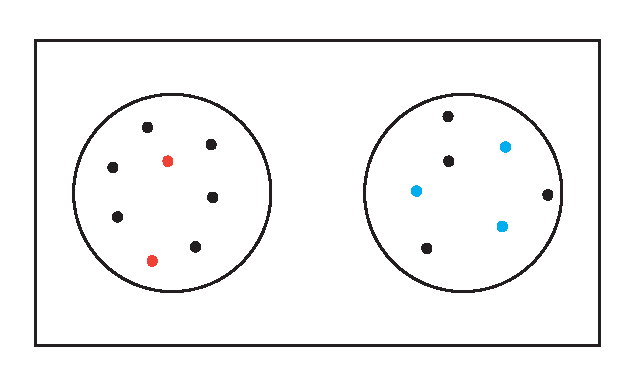
\includegraphics{sigmastructure.pdf}

A $\Sigma$-structure
\end{center}

  

\end{frame}


\begin{frame}

\begin{itemize}
\item there is a unique $x$ of sort $s_1$ that is $p$.
\item there is a unique $y$ sort $s_2$ that is $q$.
\end{itemize}

\bigskip
A $\Sigma$-theory $T$

\end{frame}

\begin{frame}

 \begin{center}
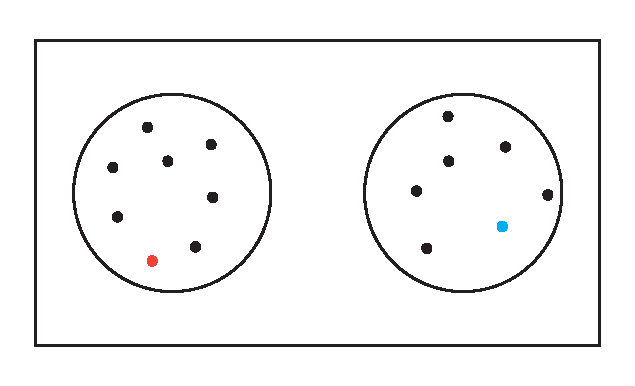
\includegraphics{Tmodel.pdf}

A model of the $\Sigma$-theory $T$
\end{center}


\end{frame}

\begin{frame}

Two theories are \textbf{logically equivalent} if they have the same
class of models. \end{frame}

\begin{frame}

\begin{itemize}
\item there is a unique $x$ of sort $s_1$ that is $p$ and there is a
  unique $y$ of sort $s_2$ that is $q$.
\end{itemize}

\bigskip
A theory $T'$ that is logically equivalent to $T$


\end{frame}


\begin{frame}

There are many pairs of theories that are not logically equivalent,
but are nonetheless intuitively equivalent.  

\end{frame}


\begin{frame}

\begin{itemize}
\item Linear orderings in signature $\{ \leq \}$.
\item Linear orderings in signature $\{ < \}$.
\end{itemize}

\end{frame}


\begin{frame}
\begin{itemize}
\item The theory that says, ``there is a $p$'', in the signature $\{ p
  \}$.
\item The theory that says, ``there is a $q$'', in the signature $\{ q
  \}$.
\end{itemize}

\end{frame}

\begin{frame}

A \textbf{definitional extension} of a theory $T$ is a theory $T^+$
obtained by adding to $T$ definitions of new predicate symbols,
function symbols, and constant symbols. 

\end{frame}


\begin{frame}

Example: ZFC formalized in $\{ \in \}$.  Define a relation $\subseteq$
by 
$$ (x\subseteq y )\: \leftrightarrow \: \forall z(z\in x\to z\in y) .$$


\end{frame}


\begin{frame}

Two theories are \textbf{definitionally equivalent} if they have a
common definitional extension. \end{frame}


\begin{frame} There are pairs of theories that are not definitionally
  equivalent, but are nonetheless intuitively equivalent. \end{frame}

\begin{frame}

\begin{itemize}
\item The empty theory in signature $\{ s_1,s_2\}$.
\item The theory in signature $\{ s,p,q\}$ that says there is an $x$
  that is $p$, a $y$ that is $q$, and every $z$ is either $p$ or $q$
  but not both.
\end{itemize}

\end{frame}


\begin{frame}

 \begin{center}
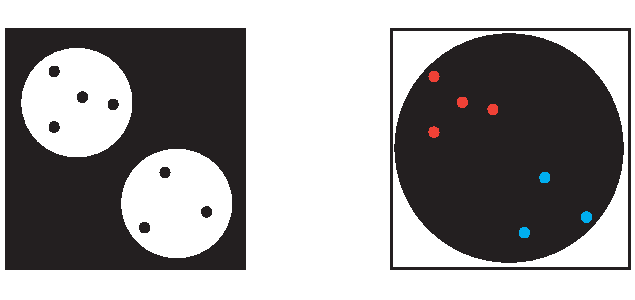
\includegraphics{quineexamplemodels.pdf}

models of these two theories
\end{center}

\end{frame}

\begin{frame}

A \textbf{Morita extension} of a theory $T$ is a theory $T^+$ obtained
by adding to $T$ definitions of new sort symbols, relation symbols,
function symbols, and constant symbols. 

\end{frame}

\begin{frame}

Two theories are \textbf{Morita equivalent} if they have a common
Morita extension. 

\end{frame}

\begin{frame}{Realism without naivete}

\begin{itemize}
\item $\Sigma = \{ s\}$.  $T$ says that there are exactly two things.
\item $\Sigma = \{ s_1,s_2 \}$.  $T'$ says that there are two things
  of type $s_1$, and four things of type $s_2$.  Things of type $s_2$
  are ordered pairs of things of type $s_1$.
\end{itemize}


\end{frame}



\begin{frame}

  \emph{Unfortunately}, Morita equivalence doesn't generalize directly
  to theories beyond the ambit of first-order logic.  \end{frame}

\begin{frame}

\begin{itemize}
\item First order theories have categories of models.
\item Physical theories have categories of models too. 
\end{itemize}

\end{frame}

\begin{frame}

\begin{center}
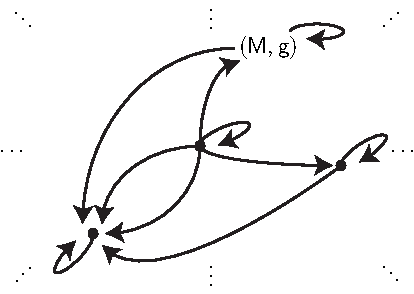
\includegraphics{grcategory.pdf}

The category of models for general relativity
\end{center}

\end{frame}


\begin{frame}

  Two theories are \textbf{categorically equivalent} if they have
  equivalent (structurally identical) categories of
  models. \end{frame}


\begin{frame}

\textbf{Theorem 1.} If two theories are Morita equivalent, then they
are categorically equivalent. \end{frame}


\begin{frame}

  \textbf{Theorem 2.} There are categorically equivalent theories that
  are not Morita equivalent. \end{frame}


\begin{frame}{The disappearance of structure?}

\begin{center}
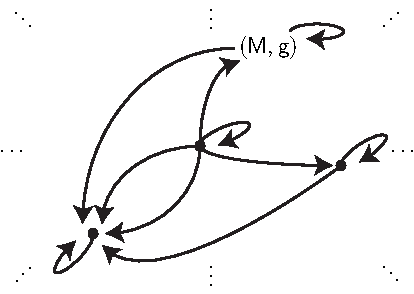
\includegraphics{grcategory.pdf}

The category of models for general relativity
\end{center}

\end{frame}



\end{document}
%%% Local Variables:
%%% mode: latex
%%% TeX-master: t
%%% End:
